% latex file for generating the development notes

\documentclass{article}

\usepackage{cite}% Make references as [1-4], not [1,2,3,4]
\usepackage{url}  % Formatting web addresses 
\usepackage{amsmath}
\usepackage{amssymb}
\usepackage{epsfig}


% Article top matter
\title{yeast\_MFC Developer Notes} %\LaTeX is a macro for printing the Latex logo
\author{Ryan Tasseff, \texttt{rtasseff@systemsbiolgy.org}}  %\texttt formats the text to a typewriter style font
\date{\today}  %\today is replaced with the current date



\begin{document}

\maketitle


\begin{abstract}
Detailed notes of the development of the yeast microfludic chip model,
using the Biocellion framework.
The model will capture the behavior of 
budding yeast and the surrounding environment in a chip designed 
designed to trap single yeast cells for time laps imaging.
Here we track the development of the model over time.
A loose organizational scheme is used, with components then function then time.
The document is dynamic will will change and the project progresses. \end{abstract}
 
\section{Introduction}
Here we will cover the development of the yeast microfludic chip model,
using the Biocellion framework.
The primary goal of the model is to capture the behavior of 
budding yeast and the surrounding environment in a chip  
designed to trap single yeast cells for time laps imaging.
Specifically, we wish to model simple aspect of yeast: 
movement, budding/ division, death and nutrient uptake.
We also want to capture the diffusion and (if needed) the 
convection/ advection of key molecules, 
to model there spatial distribution over time.

The following is a rough guide to how the model was/ is being developed.
There is no specific structure; however, 
we will attempt to organize first by specific model components, 
then by relevant biology/ function and finally by date (time stamp on all additions).
To some extent, we will leave deprecated code/ descriptions
in the notes; however, we will try to mark them as deprecated.

\section{General Assumptions, Simplifications and Implementation Details}
\subsection{Units}
time = seconds (sec);
length = micrometers ($\mu m$);
volume = cubic micrometers ($\mu m^3$);
mass = micro grams ($\mu g$);
concentration = $frac\{\mu g}{\mu m^3}$;

\subsection{Growth and Division}
\emph{20131111} We are assuming a simple model of growth, division and cell cycle control\cite{Charvin2009}.
The primary assumptions are 1) exponential growth of cells
2) perfect volume control,
the cells do not start a clock until some $V_C$ is reached;
2b) all additional volume will be transfered to daughter;
3) linear progression through cell cycle;
3b) completely deterministic mitosis, 
the cell finishes division after clock hits 1.
Currently, we have added some additional simplification and assumptions:
\emph{20131125}
Previous division replaced by budding.
Budding assumed to start based on \cite{Charvin2009} at .25.
All volume donated to bud.
In this model, a bud is an independent agent,
and is connected to the mother by a junction end.
Currently the bud direction is monitored in the cell.
This is the place where each daughter will bud from.
In actuality the bud location moves slightly, but that is not captured here.
Rotation will be included to allow for rotation of the bud direction.
Daughter bud direction will be set opposite to mother upon bud formation, similar to actual observation.
Linked mother daughters will have a spring potential that holds them together.
Currently we do not have a force model for rotation,
we simply track the direction for future use. 
The direction for the bud should always be such the direction vector that joins the mother daughter centers.
This will be the only form of rotation in the model, at this time.


\subsection{Physical Environment}
\emph{20131111} Although the model does contain 3 dimensions,
we will focus only on the first 2 (x,y), 
and assume movement is restricted in z-axis based on chip size.
This assumption should be naturally enforced if we make no movement in z-axis.
\textbf{NOTE:} This obviously will not account for any forces due to the z-axis,
for example making the width smaller will not increase friction and will not effect particle movement at all.
\emph{20131112} Because we will be using a complex shape we will have to define special regions.
Currently regions can be defined as uninhabitable, and no agents will be allowed in, and
as PDE and pde diffusion at interface will be manually set to zero.
\textbf{NOTE:} While PDE buffer MAY be enough to constrain molecules we will need more with agents.
We should find a way to see if the box is uninhabitable, 
implement shoving and perhaps even friction and rotational forces.

The shape of the trial system will be modeled after figure \ref{FIG:chip}.
The x-axis will be along the horizontal, 
which is perpendicular to the flow channel.
The chip is modeled at the scale of a unitbox (close to the size of a single cell).
The unitbox will be defined as open (1) or closed (0) via a design matrix,
and this will be used to setup habitability, diffusion and other constants.
therefore, the x-boundary conditions for diffusive molecules will be Dirchlet.
They will be set to maintain the same concentration in the channel itself.
Other boundaries will be Numman assuming no flux through walls.

\subsection{Nutrient Constraints}
\label{S:nutriant}
\emph{20131111} We will assume that nutrients is required for growth and division.
Currently we treat glucose as only required nutrient.
We assume uptake is constant.
Estimates were provided by Gilles Lab to be an uptake of
$2.5E-12 \frac{g}{min*cell}$ which comes out to 4.17E-2 $\frac{pg}{sec*cell}$.
The bulk concentration in the flow channel is $20\frac{g}{L}$ which comes to 2E-2 $frac\{pg}{\mu m^3}$.

\subsection{Diffusion}
Currently we are assuming that only diffusion exists for transport of species in the environment.
This should be close to true in the channel, as the low rynolds number should prevent advection due to flow at the boundary.
The model calculates flux as so:
\begin{equation}
J = D ( \frac{\phi_0}{\kappa_0} - \frac{\phi_1}{\kappa_1} ) \frac{1}{h}
\label{EQ:diff}
\end{equation}

We will set diffusion coefficients to zero at walls of the chip,
and we will use dirchlet (constant concentration) boundary conditions for the flow channel.


\subsection{Uptake}
Calculating nutrient uptake at the agent level only produces errors, as uptake is too high when multiple agents are present.
Here we have used a strategy to calculate the total uptake for a grid by all agents using updateGridVars.
That is the logic needs to be known for grid updates, not the agent.
We then set a variable indicating what fraction of needed uptake is available,
the delta or sink term is also calculated here to reflect this fraction.
The logic to determine agent uptake is quite simple and basically assumes uptake is proportional to cell volume;
reasonable given that growth is exponential.
We note that a lower limit has been set on total uptake from a grid,
that is you cannot take everything from a gird.
This is a relative limit so at low levels the cell uptake follows first order kinetics.
Together this is similar to saturation kinetics.
\textbf{NOTE:} One additional approximation is for cells bound by a bud.
For the gird, uptake is assumed to take place based on where the cells are, independently;
however, for growth, the daughter agent grows wrt volume of each bound cell, 
and the amount available is based on the daughters location.
This simplifies complex communications between the mother and daughter.
If mother and daughter exist in grids with similar nutrient levels, 
this will have minimal impact;
otherwise, cells will grow disproportionally to the uptake.
\textbf{NOTE:} We could also include a rough estimation of the diffusion into/out of the current location.  
Currently the max time step is limited to what is required for resolving movement, not uptake.


\subsection{Mechanical Forces and Interactions}
Currently, as mentioned above, 
we have NO interactions with the walls at this moment,
except for the fact the disp is recalculated to prevent penetration.
Only agent agent shoving produces force.
Displacement will be calculated based on an overdamped system:
\begin{equation}
\dot{x} = \frac{1}{c} \sum F
\label{EQ:disp}
\end{equation}
where $c$ is the friction coefficient and $F$ is the force, the dot denotes change with respect to time.
Here a simple finite difference model is used to calculate delta x.

\subsection{Occupation Fraction}
\emph{20131210}
SK has developed a new method to identify the occupation fraction of a sphere in a unit box.
This method is quick and now standard so we will employ it here.
We will call the calculation in both the \textit{updateSpAgentState()} and the \textit{updateIfGridVar} methods.
For simplicity, we will not save fractions to model variables.
The method subdivides the UB into grids to do the calculation,
we are using level 4 which is a $16^3$ subdivision of the UB. 
\textbf{NOTE:} The down side is that the current method does not redistribute volume 
in uninhabitable areas to habitable ones.
For example if a yeast cell is technically overlapping an uninhabitable area,
one interpretation is that it is being deformed, but the volume exclusion remains the same.
In this case we could redistribute volume to habitable areas.  
Without doing this, we are assume a deformation of the domain that is not constant wrt volume.
This will throw off calculations like how much uptake an agent has if it is overlapping an uninhabitable area.
A fix would be to calculate on all surrounding grids then renormalise all fractions.
This requires additional calculations, 
especially in the grid update step where neighbor fractions are not directly used.
We will not implement this unless necessary.

\textbf{Old Method, Dpericated on 20131210-->:}
Each agent's position is defined by a single point.  
In this simulation, using spheres, we take this point as the center.
Because the agents have non zeros volumes they occupy space in the unit boxes (UB).
While the center is defined in a single UB its likely that the agent overlaps neighbor UBs.
With larger UBs or less packed systems over larger domains approximating an agent to a single UB may be acceptable,
here we found it necessary to identify the fraction of overlap in each UB.
The primary issue is dealing with volume exclusion,
in some cases 2 agents enter a UB at the same step, 
which will drastically and suddenly increases the excluded volume and cause errors in the PDE.
This is artificial due to the discrete nature of assigning the full volume to a single UB.
Here we approximate the fraction of volume in all neighbor UBs.
A complete solution is quite cumbersome so here we use an approximation.
Recall that the grid is regular and square with an edge length => the diameter of the largest agent.
Here we identify the overlap with neighboring UB's in much the same way as done for estimating physical interactions.
We find the shortest distance from the agent center to the boundary of the neighbor UB, $d$.
This is the distance to the edge of immediate neighbors and the corner of corner neighbors.
We then compare this to the radius, $r$.
If $r>d$, the overlap distance is $\delta = r-d$, and zero otherwise.
This gives us the overlap with each neighbor.  
We define the effective internal distance as:
\begin{equation}
\delta_0 = (1+n)*r - \sum_i \delta_i,
\end{equation}
where $n$ is the number of overlapping neighbors and the sum is carried out over these neighbors.
This was chosen so that the situation of equally overlap of an agent being on an edge between two UBs ($n=1$) or 
at a corner between 4 UBs ($n=3$) $\delta_0=\delta_i$.
The total is taken as the sum of all $\delta$ adn fractions for each overlap are calculated.
This fraction is used as the occupation fraction and is used to divide quantities, like volume, over multiple UBs.
The solution has 3 primary characteristics: 
(1) it is consistent in the sense that a UB is estimated to have agent overlap iff it actually has overlap,
this is not meant to imply the formal numerical concept of consistency although it may;
(2) it is continuous up to the step size, this mean that as an agent travels into a new UB 
its volume fraction will grow in increments from zero, 
where these increments can be made arbitrarily small by reducing the time step;
(3) it conserves the quantities being shared, 
since we approximate a fraction for each UB and force the total to be one by definition 
any quantity shared over the UBs using this fraction will remain constant over all UBs.
We also note that it is exact in some situations as described above.
\textbf{:<--Old Method, Dpericated on 20131210}


\section{Initialization}
\emph{20130927} We have initialized the model using the PDE example provided in Biocellion.

\section{Model Properties and Definitions}
The following is a general overview of the various elements on the model.
Nearly all is defined in model \textit{model\_define.h}.

\subsection{Agent types and properties}
\emph{20130927} We will add agents under `---Agents---'.
The primary agent is \texttt{AGENT\_YEAST\_CELL}.
We also added the initial properties in the same place,
specifically we have added 2 model reals that describe the 
location of the budding direction \texttt{YEAST\_CELL\_MODEL\_REAL\_BUD\_DIR\_}.
\emph{20130927} The property \texttt{YEAST\_CELL\_MODEL\_REAL\_CC\_CLOCK}
was added to monitor progression through the cell cycle \cite{Charvin2009}
Additional cell properties added under `---Cell Properties--- including 
`-Growth and Division-' properties taken from \cite{Charvin2009} to describe the cell cycle.

Uptake of diffusible elements is also possible,
Standard constant values are being used for this first impl using \texttt{CELL\_ELEM\_CONSTANT\_UPTAKE}.
Currently we have only one element so its a real, 
but we should change to array if more are added.
This would be reflected under `---Diffusible elements---'.
Estimate was provided as above in \ref{S:nutriant}.
As for diffusion we are assuming a constant, except at boundaries,
and assuming the solvent is water.
The diffusion coef for glucose was found to be 600 $\frac{\mu m^2}{sec}$,
found in bionumbers.hms.harvard.edu.



\subsection{Grid Properties} 
Props found under `---Grid Properties---'.

The flow channel is modeled by constant concentration boundary conditions, 
these are set in \texttt{ELEM\_BULK\_CONCENTRATION}.
Currently we have only one element so its a real, 
but we should change to array if more are added.
This would be reflected under `---Diffusible elements---'.
Estimate was provided as above in \ref{S:nutriant}. 


\subsection{Domain}
\emph{20131113} Under `---Domain---'
Unit box size \texttt{IF\_GRID\_SPACING} is set to maximum interaction dist 
\texttt{CELL\_INTRCT\_DIST\_MAX} which is the cell diameter of the largest cell.
Currently we assume that the largest cell is double the critical volume,
and critical volume corresponds to a sphere with 2 $\mu$m radius (estimate).
\textbf{NOTE:} Once budding is introduced cells will not grow very large before division,
and we can reduce the maximum size and the grid spaces will also reduce.

Design of the domain is given by \texttt{CHIP\_DESIGN\_MATRIX}, 
entries are zero and one.
One indicates a habitable region, only z=0 is habitable.





\section{Agent Rules}
Rules defined in \textit{model\_routine\_agent.cpp} unless otherwise stated.

\subsection{updateSpAgent}
\emph{20131111} We define growth here.  
Currently, we have deterministic exponential volume increase.
Which is achieved by simple steps.  
\emph{20131113} Moved cell cycle to here to connect with uptake.
Here have track movement through the cell cycle by linearly increasing the phase variable under ` ---Cell Cycle Progression---'.
Both growth and cell cycle progression only occur if enough glucose is available.
We calculate the total amount of nutrients in the box and the needs,
if enough is present we set a model real, \texttt{YEAST\_CELL\_MODEL\_REAL\_ELEM\_GLUCOSE\_UPTAKE},
to the amount we expect to take for this step and we allow growth and clock to update.



\subsection{updateSpAgentBirthDeath }
\emph{20131111} We are doing all division at a single step,
as opposed to a bud.
So when cell cycle is complete we allow the cells to divide.
Based on \cite{Charvin2009} cell cycle is complete after the clock reaches 1.0.
The limit is defined in \textit{model\_define.h} as \texttt{CC\_CLOCK\_CRITICAL}.
We note that the phase is tracked as an internal variable \texttt{YEAST\_CELL\_MODEL\_REAL\_CC\_CLOCK}

\subsection{adjustSpAgentState}
\emph{20131111} Very simple model to calculate velocity based on EQ \ref{EQ:disp}.
Finite difference gets us from velocity to displacement.
Added under `---DISP---'.

\subsection{divideSpAgent}
\emph{20131111} Division is done all at once.  
After the cell cycle is complete this method will be called.
All volume above the critical volume is sent to the daughter.
Displacement is done so that both move to account for new radius, 
and this is in the direction of the budding, defined as a property in \textit{model\_define.h}.
 

\section{Mechanical Interactions}
Rules defined in \textit{model\_routine\_mech\_intrct.cpp} unless otherwise stated.

\emph{20131112} Standard force will be calculated based on shoving only.
Shoving is basically like the positive potential part of the spring potential,
The spring constant is the cell stiffness \texttt{CELL\_STIFF}, 
which defined in \textit{model\_define.h} and set to allow 50\% of total disp from shoving.


\section{Grid Updates and Init}
Rules defined in \textit{model\_routine\_grid.cpp} unless otherwise stated.

\emph{20131122} 
\subsection{initIfGridVar}
Initialize all properties at zero.

\subsection{updateIfGridVar}
Uptake of nutriants is done here. 
The strategy is to go through all cells and identify the total amount they have used in a grid variable \texttt{GRID\_MODEL\_REAL\_GLUCOSE\_DELTA}.
This will be passed to the section that updates the RHS or source term.
Note that what the sign is opposite from the agent variable, \texttt{GRID\_MODEL\_REAL\_GLUCOSE\_DELTA}, 
to the agent from the environment.

Here we add up the agent volume in this grid.
This is then stored in \texttt{GRID\_MODEL\_REAL\_AGENT\_VOL} for latter use.

\subsection{updateIfGridKappa}


The model tracks the concentration as the amount (conserved quantity) over the volume of the UB.
However, the actuall volume accessable can be reduced by cells, 
so that the effective concentration (for the same ammount) is higher.
Here we are using mass as the conserved quantity, specifically for glucose,
and we need to correct the concentrations used in calcualting the flux based on the excluded cell volume.
Here we use \texttt{GRID\_MODEL\_REAL\_AGENT\_VOL}, set above, 
to calculate the correction factor.
This will be set the $\kappa_i$ in eq \ref{EQ:diff}.
We will limit this to 0.01 defined by \texttt{KAPPA\_MIN}.
Very small values cause huges changes in flux and are not advised.
We note that currently all the volume of an agent is assumed to be excluded from the UB that contains the agent's center.
We do not calculate the volume in neighbor UBs, so its possible to take up more volume then the UB has.

\subsection{updateIfGridBetaInIfRegion and updateIfGridBetaDomainBdry}
Here we set the diffusion coefficient for each grid interface.
To prevent diffusion into the uninhabitable area, 
we only assign non zero diffusion to interfaces between 2 habitable UBs.

Here we also calculate an effective diffusion.
In eq \ref{EQ:diff} we see that the flux is calculated based on model params;
however, the amount of conserved quantity (in this case mass) that is transfered is calculated using the full available area: $J*h^2$.
The area for flux may be reduced, excluded, due to cells in the way.
We cannot change the area used to calculate transfer,
but we can modify $D$ to equivalently compensate for reduced area.
To do this we scale $D$ by the amount fraction of volume available.
This is done for each UB separately, and the harmonic mean,
as suggested by SK, was used to combine them for the $D$ at the interface.

A similar strategy was used at the boundaries modeling the flow channel.
Here we have dirchlet boundary conditions on all x walls,
and in this method we set all diffusion at boundaries to 0, except 
in x directions AND when we are at a habitable, non chip wall, area.
 
All other betas are set to zero!

\subsection{updateIfGridRHSLinear)
Here is where we update the source term for the grid UB.
This is the chance we have to complete the cell uptake.
Using the previously, \textit{updateIfGridVar}, set variable, \texttt{GRID\_MODEL\_REAL\_GLUCOSE\_DELTA}.  
First we consider how much was taken from this grid UB, 
if it was too much then we screwed up, but we cannot fix that now,
so just set it to take everything from the box.
Note that a warning can be printed when this happens, 
to fix the issue of taking to much use smaller grid state step sizes.
When removing the mass, it is done continuously while the PDE is solved,
this means we need to calculate the source term, which is change/ (volume * time step ).





\begin{figure}
\begin{center}
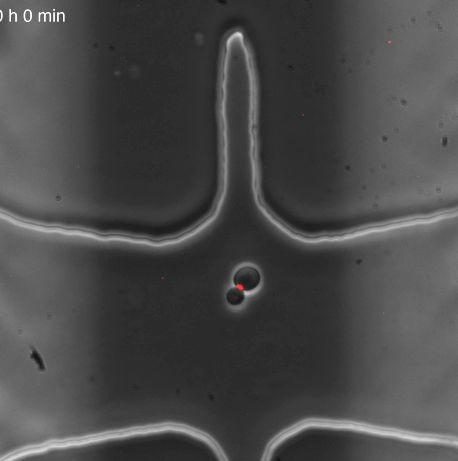
\includegraphics{figs/chip.png}
\caption{Screen shot of loaded chip.  
Flow channels are on the left and right (out of frame).
The model will simulate x-axis along or parallel to the horizontal of this image, 
and y-axis along or parallel to the vertical.}
\label{FIG:chip}
\end{center}
\end{figure}







\bibliographystyle{plain}
\bibliography{mainRefDB}

\end{document}  %End of document.
